\documentclass[12pt,letterpaper]{article}

\usepackage{fancyhdr}
\pagestyle{fancy}
\fancyhf{}
\rhead{Vaja 4}
\lhead{ORS}
\setlength{\headheight}{16pt}

\usepackage[utf8]{inputenc}
\usepackage[slovene]{babel}
\usepackage[colorlinks = true, urlcolor = blue]{hyperref}

\usepackage{xcolor}
\usepackage{listings}
\usepackage{graphicx}
\graphicspath{{./images/}}
\definecolor{mGreen}{rgb}{0,0.6,0}
\definecolor{mGray}{rgb}{0.5,0.5,0.5}
\definecolor{mPurple}{rgb}{0.58,0,0.82}
\definecolor{backgroundColour}{rgb}{1,1,1}

\lstdefinestyle{CStyle}{
    backgroundcolor=\color{backgroundColour},   
    commentstyle=\color{mGreen},
    keywordstyle=\color{magenta},
    numberstyle=\tiny\color{mGray},
    stringstyle=\color{mPurple},
    basicstyle=\footnotesize,
    breakatwhitespace=false,         
    breaklines=true,                 
    captionpos=b,                    
    keepspaces=true,                 
    numbers=left,                    
    numbersep=5pt,                  
    showspaces=false,                
    showstringspaces=false,
    showtabs=false,                  
    tabsize=2,
    language=C,
    frame=none
}

\begin{document}

\begin{center}
    \textbf{\Large Uporaba STM HAL knjižnice za delo s splošno namenskim vhodom/izhodom}   
\end{center}

Na tokratni vaji bomo spoznali še tretji in zadnji način razvoja programske opreme za mikrokrmilnike. Prvi je bil neposredno pisanje na naslove, drugi pa priprava lastnih funkcij oziroma knjižnice za delo z GPIO napravami. Tokrat bomo spoznali še knjižnico, ki jo ponuja proizvajalec mikrokrmilnika. Knjižnica je narejena na podoben način kot tista, ki ste jo začeli graditi na zadnji vaji. Razlika je le v tem, da proizvajalčeva knjižnica podpira vse funkcionalnosti vseh naprav na mikrokrmilniku in da to knjižnico uporablja milijone razvijalcev po svetu in je tako možnost za hrošče bistveno manjša. Knjižnica, ki jo je razvil proizvajalec mikrokrmilnika, se imenuje HAL Driver Library oziroma krajše HAL. Glavnina datotek knjižnice se nahaja v mapi \texttt{Drivers/STM32F4xx\_HAL\_Driver}. Tu najdete dve podmapi, \texttt{src}, kjer se nahajajo .c datoteke s funkcijami ter \texttt{inc} s .h datotekami, kjer najdemo konstante in prototipe funkcij.

Prvi del knjižnice, ki ga bomo spoznali na tokratni vaji, omogoča delo z digitalnim vhodom in izhodom, torej z GPIO napravami.


\section*{Vklop ure GPIO naprave}

Podobno kot na zadnji vaji, bomo tudi tokrat začeli z vklopom ure GPIO naprav. Za ta namen ste na zadnji vaji razvili funkcijo \texttt{clock\_on()}. HAL knjižnica ponuja za ta namen več funkcij, vsako za eno izmed GPIO naprav. Funkcija \texttt{\_\_HAL\_RCC\_GPIOA\_CLK\_ENABLE()} tako vklopi uro naprave GPIOA, \texttt{\_\_HAL\_RCC\_GPIOB\_CLK\_ENABLE()} vklopi uro naprave GPIOB in tako naprej do \texttt{\_\_HAL\_RCC\_GPIOI\_CLK\_ENABLE()}, ki vklopi uro naprave GPIOI. Takšne skupine funkcij običajno krajše zapišemo z \texttt{\_\_HAL\_RCC\_GPIOx\_CLK\_ENABLE()}, kjer \texttt{x} nadomestimo s črkami A do I. Definicije teh funkcij se nahajajo v datotekah \texttt{stm32f4xx\_hal\_rcc.h} ter \texttt{stm32f4xx\_hal\_rcc\_ex.h}.

HAL ponuja še funkcije za izklop ure, \texttt{\_\_HAL\_RCC\_GPIOx\_CLK\_DISABLE()} ter funkcije, ki določajo kaj se dogaja z urami GPIO naprav, ko mikrokrmilnik preklopimo v način delovanja, ki omogoča nižjo porabo energije (angl. Low Power Mode). To sta funkciji \texttt{\_\_HAL\_RCC\_GPIOx\_CLK\_SLEEP\_ENABLE()} in \texttt{\_\_HAL\_RCC\_GPIOx\_CLK\_SLEEP\_DISABLE()}.


\section*{Inicializacija GPIO naprave}

Pri knjižnic HAL za inicializacijo uporabljamo funkcijo \texttt{HAL\_GPIO\_Init}. Ta sprejme dva parametra, kazalec na strukturo \texttt{GPIO\_TypeDef} ter kazalec na strukturo \texttt{GPIO\_InitTypeDef}. V datoteki \texttt{stm32f407.h} je definirana struktura \texttt{GPIO\_TypeDef}, ki je prikazana spodaj.

\begin{center}
\begin{lstlisting}[style=CStyle]
typedef struct
{
  __IO uint32_t MODER;
  __IO uint32_t OTYPER;
  __IO uint32_t OSPEEDR;
  __IO uint32_t PUPDR;
  __IO uint32_t IDR;
  __IO uint32_t ODR;
  __IO uint32_t BSRR;
  __IO uint32_t LCKR;
  __IO uint32_t AFR[2];
} GPIO_TypeDef;
\end{lstlisting}
\end{center}

Ta struktura bi vam morala biti bolj ali manj že poznana, saj smo podobno strukturo zgradili že pri zadnji vaji. Opazimo pa lahko tri razlike. Prva je, da imajo vsi elementi predpono \texttt{\_\_IO}, gre zgolj za preimenovano rezervirano besedo \texttt{volatile}. V naši knjižnici smo to izpustili, je pa za pomnilniško preslikane lokacije (registre) dobra praksa, da se spremenljivkam dodeli status \texttt{volatile}. Druga razlika je, da sta tu registra \texttt{Bit Set} in \texttt{Bit Reset} združena v register \texttt{Bit Set Reset (BSRR)}. Knjižnica tako namesto dveh registrov uporablja zgornjo in spodnjo polovico večjega registra. Tretja in zadnja razlika so dodatni registri: \texttt{LCKR} omogoča zaklep nastavitev, \texttt{AFR[0]} in \texttt{AFR[1]} pa omogočata nastavitve alternativnih funkcij, kadar pinu določimo ta način delovanja. Pri naši prejšnji vaji smo jih izpustili, ker jih nismo potrebovali.

V datoteki \texttt{stm32f407.h} najdemo tudi naslednje konstante:

\begin{center}
\begin{lstlisting}[style=CStyle]
#define GPIOA               ((GPIO_TypeDef *) GPIOA_BASE)
#define GPIOB               ((GPIO_TypeDef *) GPIOB_BASE)
#define GPIOC               ((GPIO_TypeDef *) GPIOC_BASE)
#define GPIOD               ((GPIO_TypeDef *) GPIOD_BASE)
#define GPIOE               ((GPIO_TypeDef *) GPIOE_BASE)
#define GPIOF               ((GPIO_TypeDef *) GPIOF_BASE)
#define GPIOG               ((GPIO_TypeDef *) GPIOG_BASE)
#define GPIOH               ((GPIO_TypeDef *) GPIOH_BASE)
#define GPIOI               ((GPIO_TypeDef *) GPIOI_BASE)
\end{lstlisting}
\end{center}

Tudi takšen zapis konstant bi vam moral biti že znan. V vaših knjižnicah ste uporabili konstante \texttt{GPIOAd, GPIOBd, ..., GPIOId}. Črko d smo dodali razno zato, da ni bilo konfliktov z že definiranimi konstantami. Pri vaših knjižnicah ste namesto imen \texttt{GPIOD\_BASE} zapisali kar neposredne naslove. Tu je vse skupaj zgradeno modularno, če pogledamo na primeru \texttt{GPIOD}:

\begin{center}
\begin{lstlisting}[style=CStyle]
#define PERIPH_BASE           0x40000000UL

#define AHB1PERIPH_BASE       (PERIPH_BASE + 0x00020000UL)

#define GPIOD_BASE            (AHB1PERIPH_BASE + 0x0C00UL)

#define GPIOD               ((GPIO_TypeDef *) GPIOD_BASE)
\end{lstlisting}
\end{center}

Če ročno izračunamo naslove dobimo \texttt{GPIOD = 0x40020C00}, kar je enaka vrednost, kot ste jo uporabili v vaših knjižnicah. 

Prvi argument funkcije \texttt{HAL\_GPIO\_Init} je tako konstanta \texttt{GPIOx}, podobno kot pri funkciji \texttt{init\_GPIO()} iz prejšnje vaje. Namesto preostalih petih argumentov naše funkcije imamo pri HAL zgolj enega. Kot že rečeno, gre za kazalec na strukturo \texttt{GPIO\_InitTypeDef}. V to strukturo zapišemo želene nastavitve pinov, ki jih funkcija \texttt{HAL\_GPIO\_Init} nato preslika v registre, podobno kot so to počele vaše funkcije v zadnji nalogi. Struktura \texttt{GPIO\_InitTypeDef} je definirana v datoteki \texttt{stm32f4xx\_hal\_gpio.h}:

\begin{center}
\begin{lstlisting}[style=CStyle]
typedef struct
{
  uint32_t Pin;  /*!< Specifies the GPIO pins to be configured. This parameter can be any value of @ref GPIO_pins_define */
  uint32_t Mode;      /*!< Specifies the operating mode for the selected pins. This parameter can be a value of @ref GPIO_mode_define */
  uint32_t Pull;      /*!< Specifies the Pull-up or Pull-Down activation for the selected pins. This parameter can be a value of @ref GPIO_pull_define */
  uint32_t Speed;     /*!< Specifies the speed for the selected pins. This parameter can be a value of @ref GPIO_speed_define */
  uint32_t Alternate;  /*!< Peripheral to be connected to the selected pins. This parameter can be a value of @ref GPIO_Alternate_function_selection */
}GPIO_InitTypeDef;
\end{lstlisting}
\end{center}

Struktura ima torej 5 elementov, s katerimi določimo nastavitve za inicializacijo naprave. Vsak izmed elementov ima omejen nabor vrednosti, ki mu jih lahko določimo. V komentarju je za vsakega zapisano ime nabora vrednosti, ki jih lahko uporabimo (\texttt{GPIO\_pins\_define}, \texttt{GPIO\_mode\_define}, ...).

\subsection*{Mode}

Nabor možnih vrednosti za element \texttt{Mode} je:

\begin{center}
\begin{lstlisting}[style=CStyle]
#define  GPIO_MODE_INPUT                        0x00000000U
#define  GPIO_MODE_OUTPUT_PP                    0x00000001U
#define  GPIO_MODE_OUTPUT_OD                    0x00000011U
#define  GPIO_MODE_AF_PP                        0x00000002U
#define  GPIO_MODE_AF_OD                        0x00000012U
#define  GPIO_MODE_ANALOG                       0x00000003U
\end{lstlisting}
\end{center}

V primerjavi z vašimi funkcijami, tu z elementom \texttt{Mode} ne določimo zgolj načina delovanja ampak, v primeru, da uporabimo izhodni način delovanja, določimo tudi tip izhoda (push-pull/open-drain). Isto velja za alternativne funkcije.

\subsection*{Speed}

Nabor možnih vrednost za element \texttt{Speed} je:

\begin{center}
\begin{lstlisting}[style=CStyle]
#define  GPIO_SPEED_FREQ_LOW         0x00000000U
#define  GPIO_SPEED_FREQ_MEDIUM      0x00000001U
#define  GPIO_SPEED_FREQ_HIGH        0x00000002U
#define  GPIO_SPEED_FREQ_VERY_HIGH   0x00000003U
\end{lstlisting}
\end{center}

Tukaj knjižnica namesto številčnih  (2MHz, 25MHz, 50MHz, ...) uporablja opisna imena. Opisna imena uporablja zato, ker knjižnica deluje z različnimi mikrokrmilniki. Pri ostalih mikrokrmilnikih hitrosti ne bodo nujno enake tem, ki jih uporablja STM32F407.

\subsection*{Pull}

Nabor možnih vrednost za element \texttt{Pull} je zapisan spodaj. Kot vidite tu knjižnica uporablja enake vrednosti, kot ste jih uporabili pri vaši rešitvi prejšnje vaje.

\begin{center}
\begin{lstlisting}[style=CStyle]
#define  GPIO_NOPULL        0x00000000U
#define  GPIO_PULLUP        0x00000001U
#define  GPIO_PULLDOWN      0x00000002U
\end{lstlisting}
\end{center}


\subsection*{Pin}

Največje razlike v primerjavi z vašimi knjižnicami se pojavijo pri naboru vrednost za \texttt{Pin}:

\begin{center}
\begin{lstlisting}[style=CStyle]
#define GPIO_PIN_0                 ((uint16_t)0x0001)
#define GPIO_PIN_1                 ((uint16_t)0x0002)
#define GPIO_PIN_2                 ((uint16_t)0x0004)
#define GPIO_PIN_3                 ((uint16_t)0x0008)
#define GPIO_PIN_4                 ((uint16_t)0x0010)
#define GPIO_PIN_5                 ((uint16_t)0x0020)
#define GPIO_PIN_6                 ((uint16_t)0x0040)
#define GPIO_PIN_7                 ((uint16_t)0x0080)
#define GPIO_PIN_8                 ((uint16_t)0x0100)
#define GPIO_PIN_9                 ((uint16_t)0x0200)
#define GPIO_PIN_10                ((uint16_t)0x0400)
#define GPIO_PIN_11                ((uint16_t)0x0800)
#define GPIO_PIN_12                ((uint16_t)0x1000)
#define GPIO_PIN_13                ((uint16_t)0x2000)
#define GPIO_PIN_14                ((uint16_t)0x4000)
#define GPIO_PIN_15                ((uint16_t)0x8000)
#define GPIO_PIN_All               ((uint16_t)0xFFFF)
\end{lstlisting}
\end{center}

Namesto številčnih oznak za pine (0, 1, 2, ...) uradna knjižnica uporablja imenske konstante, za katerimi se skrivajo zastavice. Prednost tega pristopa je, da lahko z enim klicem funkcije za inicializacijo nastavimo več pinov, medtem ko ste pri vaši knjižnici za inicializacijo LED diod potrebovali štiri klice. Primer inicializacije izhodnih pinov \texttt{PE3} in \texttt{PE6} je prikazan spodaj:

\begin{center}
\begin{lstlisting}[style=CStyle]
__HAL_RCC_GPIOE_CLK_ENABLE();

GPIO_InitTypeDef init_structure;
init_structure.Pin = GPIO_PIN_3 | GPIO_PIN_6;
init_structure.Mode = GPIO_MODE_OUTPUT_PP;
init_structure.Pull = GPIO_NOPULL;
init_structure.Speed = GPIO_SPEED_FREQ_LOW;

HAL_GPIO_Init(GPIOE, &init_structure);
\end{lstlisting}
\end{center}


\section*{Branje vhoda GPIO naprave}

HAL ima za branje vhoda na voljo funkcijo \texttt{HAL\_GPIO\_ReadPin()}. Funkciji podamo kazalec na strukturo \texttt{GPIO\_TypeDef} ter oznako pina. Primer branja vrednosti na pinu \texttt{PE3}: \texttt{HAL\_GPIO\_ReadPin(GPIOE, GPIO\_PIN\_3)}. V kodi funkcije, ki je prikazana spodaj, lahko vidite, da je implementacija branja vhoda v HAL podobna vašim implementacijam. Dodano je le nekaj preverjanj vhodnih vrednostih.

\begin{center}
\begin{lstlisting}[style=CStyle]
typedef enum
{
  GPIO_PIN_RESET = 0,
  GPIO_PIN_SET
} GPIO_PinState;

GPIO_PinState HAL_GPIO_ReadPin(GPIO_TypeDef* GPIOx,
                               uint16_t GPIO_Pin)
{
  GPIO_PinState bitstatus;

  /* Check the parameters */
  assert_param(IS_GPIO_PIN(GPIO_Pin));

  if((GPIOx->IDR & GPIO_Pin) != (uint32_t)GPIO_PIN_RESET)
  {
    bitstatus = GPIO_PIN_SET;
  }
  else
  {
    bitstatus = GPIO_PIN_RESET;
  }
  return bitstatus;
}
\end{lstlisting}
\end{center}


\section*{Nastavljanje izhoda GPIO naprave}

Za nastavljanje izhoda imamo na voljo dve funkciji: \texttt{HAL\_GPIO\_WritePin()}, ki nastavi pin na poljubno vrednost ter \texttt{HAL\_GPIO\_TogglePin()}, ki negira trenutno vrednost pina. Podobno kot pri branju, pri obeh podamo kazalec na strukturo naprave, podobno kot pri branju. Pri \texttt{HAL\_GPIO\_WritePin()} dodatno podamo \texttt{GPIO\_PIN\_RESET} (logična ničla) ter \texttt{GPIO\_PIN\_SET} (logična enica). Primeri uporabe omenjenih funkcij so prikazni spodaj:

\begin{center}
\begin{lstlisting}[style=CStyle]
HAL_GPIO_WritePin(GPIOA, GPIO_PIN_3, GPIO_PIN_RESET);
HAL_GPIO_WritePin(GPIOD, GPIO_PIN_12 | GPIO_PIN_13, GPIO_PIN_SET);
HAL_GPIO_TogglePin(GPIOA, GPIO_PIN_3);
\end{lstlisting}
\end{center}
\newpage

Kot vidite v zgornjem primeru tudi tukaj lahko nastavljamo vrednost večih pinov hkrati. Konstante \texttt{GPIO\_PIN\_X} so namreč vrednosti, ki imajo enico zgolj na pinu \texttt{X}, povsod drugje pa vrednost 0, tako lahko z logičnim ali izberemo več pinov hkrati. Pine lahko izberemo tudi tako, da vrednost parametra za izbiro pinov določimo samo, vrednost 0x7002 (binarno 0111 0000 0000 0010), bi tako izbrala pine 14, 13, 12 in 1.


\section*{Branje stanja gumba}

Zadnja tema, ki se jo bomo lotili na tej vaji, je branje gumba. Pri branju gumbov sicer zaenkrat nismo imeli bistvenih težav. Namerno se namreč nismo lotili nalog, kjer bi do težav lahko prišlo. Če pa bi s kodo iz zadnje vaje želeli implementirati števec pritiskov gumba, bi zelo hitro opazili, da bi vaša koda velikokrat zaznala več klikov gumba. Razlog tiči v fizikalnih lastnostih gumba. Namesto čistega in lepega prehoda iz ničle v enico, se namreč na vhodni liniji pojavi signal podoben temu na sliki \ref{debounce}.

\begin{figure}[ht!]
  \centering
  \caption{Napetost na vhodu ob pritisku gumba.}
  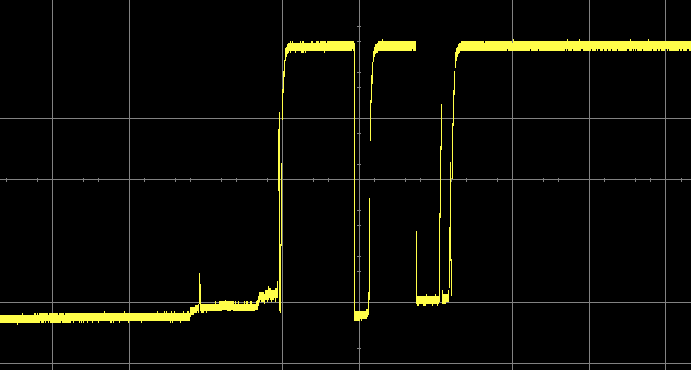
\includegraphics[height=110pt]{images/vaja4/debounce.png}
  \label{debounce}
\end{figure}

Najenostavnejša rešitev te težave, ki se ji angleško reče \textit{button debounce} je, da po tem, ko zaznamo spremembo signala iz nič v ena, počakamo preden ponovno beremo stanje gumba. Po domače povedano v naš program vstavimo zakasnitev (angl. delay). Ta je lahko zelo kratka (nekaj 10-100ms), saj napetost dokaj hitro izniha.

Psevdokoda, ki šteje število pritiskov v globalno spremenljivko vendar ne rešuje omenjene težave z debounce-om je prikazana spodaj.

\begin{center}
\begin{lstlisting}[style=CStyle]
uint8_t counter = 0;
uint8_t old = 0;
uint8_t new = 0;

while(1) {
    // preberemo novo stanje gumba
    // funkcija read_button
    new = read_button();
    
    // ce je bilo prejsnje stanje gumba 0
    // sedaj pa je 1, se je zgodil klik (prehod iz 0 v 1)
    if (old == 0 && new == 1) {
        counter++;
    }
    
    // shranimo trenutno stanje gumba kot prejsnje
    old = new;
}
\end{lstlisting}
\end{center}

\newpage


\section*{Naloga}

Realizirajte števec pritiskov na gumb. Števec naj šteje do vključno 15. Stanje števca v binarni obliki prikažite s pomočjo LED diod. Pri številu 14 (binarno 1110) naj bo prva LED dioda ugasnjena, ostale 3 pa prižgane. Pri številu 8 (binarno 1000) naj gori zgolj zadnja LED dioda. Primer štetja od 0 do 4 je prikazan na sliki \ref{LedStevec}.

\begin{figure}[ht!]
  \centering
  \caption{Prikaz vrednosti števca na LED diodah (od 0 do 4).}
  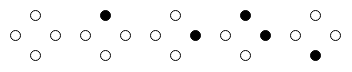
\includegraphics[width=250pt]{images/vaja4/ledstevec.png}
  \label{LedStevec}
\end{figure}

Ob kratkem pritisku gumba povečajte vrednost števca za 1, ob dolgem pritisku (2 sekundi ali več) pa nastavite vrednost števca na 0. Za implementacije morebitnih zakasnitev lahko uporabite funkcijo \texttt{HAL\_Delay(ms)}, ki ji podate število milisekund za zakasnitev. Zaznavanje dolgega klika ne sme blokirati zaznavanja kratkih klikov, torej rešitev kjer za ločevanje kratkih in dolgih klikov uporabite 2 sekundno zakasnitev ni primerna. Za izhodišče vzemite prazen projekt v razvojnem okolju.

\end{document}
